\section{\'Arbol de Decisi\'on}\label{sec:Decision_tree}
	
		Los \'arboles se utilizan en diversos campos de la inform\'atica. A pesar de que son dif\'iciles de representar y visualizar de forma global, resultan una herramienta muy \'util para separar situaciones o datos.\\
		
		La estructura de los \'arboles se puede usar con muchos fines: ordenar un vector, resolver problemas de alta complejidad computacional (como encontrar la mejor jugada posible en un tablero de ajedrez), representar redes de routers y switches o expresar la gram\'atica de un lenguaje, entre otros.\\
		
		En el caso que nos ocupa, estamos interesados en un tipo muy especial de \'arboles, los \'arboles de decisi\'on.\\
		
		\subsection{Definici\'on}
			Un grafo es un conjunto de v\'ertices y aristas. Las aristas tienen dos extremos, en cada uno de ellos se sit\'ua un v\'ertice.\\
			
			Un grafo simple es aquel que no tiene lazos (aristas cuyos extremos se conectan con el mismo v\'ertice) ni aristas m\'ultiples entre dos de sus v\'ertices.\\
			
			Un \'arbol es, pues, un grafo simple tal que
			para cada dos v\'ertices de existe un \'unico camino simple entre ellos, es decir, hay una \'unica sucesi\'on de aristas que empieza en uno de los v\'ertices y termina en el otro sin repetir arista.\\
			
			Un \'arbol de decisi\'on ser\'a, por tanto, una especializaci\'on de \'arbol en la que a los v\'ertices se los interpreta de la siguiente forma:\\
			
			\begin{itemize}
				\item Un v\'ertice especial, llamado nodo ra\'iz, se considera el inicio del camino de decisi\'on.
				\item Un conjunto de v\'ertices, llamados nodos, se conectan con, al menos, otros dos v\'ertices. En cada nodo hay una condici\'on. La verficaci\'on de dicha condici\'on determina qu\'e nodo es el siguiente en el camino de decisi\'on.
				\item Un conjunto de v\'ertices, llamados hojas o nodos terminales, se conectan con un \'unico v\'ertice. En cada hoja hay una clasificaci\'on del dato que cumple todas las condiciones que tienen los nodos del camino que empieza en la ra\'iz y termina en la hoja. 
			\end{itemize}
			
			El objetivo de un \'arbol de decisi\'on es, por tanto, clasificar datos, de una determinada naturaleza, seg\'un una serie de condiciones. La construcci\'on de dicho \'arbol y la elecci\'on de las condiciones las veremos en los siguientes apartados.\\
		
			En este punto, se procede a plantear un problema cl\'asico para dar un ejemplo de \'arbol de decisi\'on. En un campeonato de tenis al aire libre son necesarias unas buenas condiciones metereol\'ogicas. Para tomar la decisi\'on de si se puede jugar un partido, o no, se puede utilizar el \'arbol de decisi\'on de la figura \ref{fig:tenis}.
			
			\begin{figure}[H]
    			\centering
    			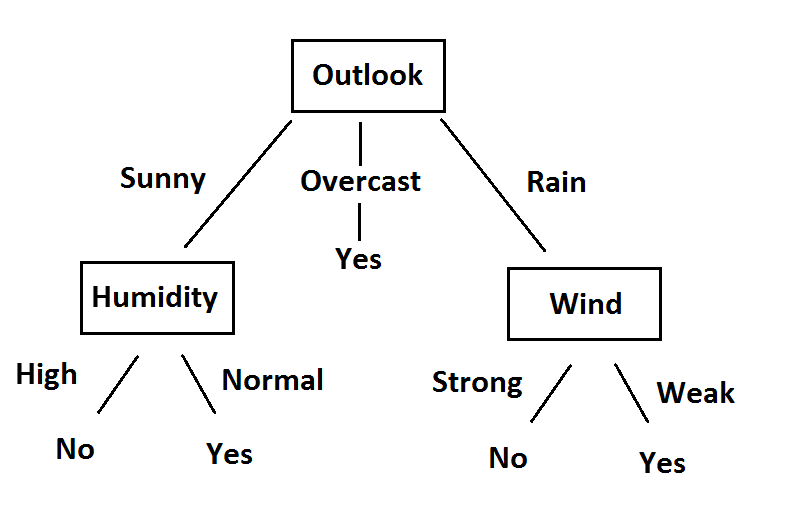
\includegraphics[scale=0.5]{imagenes/tree.png}
    			\caption[\'Arbol de decisi\'on para jugar partido de tenis.]{\'Arbol de decisi\'on para decidir si un partido de tenis se juega.\\ Fuente: \url{https://sefiks.com} [\'Ultima consulta 12 de Julio de 2019]}
    			\label{fig:tenis}
		    \end{figure}
			
			Como se puede ver, el \'arbol se interpreta del nodo ra\'iz hasta las hojas. Luego la primera condici\'on a comprobar es el estado del cielo: si est\'a nublado, entonces se juega; si por el contrario, est\'a soleado o lloviendo, entonces hay que comprobar otra condici\'on para tomar la decisi\'on.\\
			
			En este ejemplo es clara la identificaci\'on de los elementos del \'arbol de decisi\'on. La clasificaci\'on de los partidos se compone de dos etiquetas: s\'i se puede jugar y no es factible jugar. Del mismo modo, las condiciones presentes en el \'arbol son tres:\\
			
			\begin{itemize}
				\item \textbf{Situaci\'on del cielo.} Puede tomar tres valores; soleado, nublado y lluvioso.
				
				\item \textbf{Humedad.} Condici\'on que puede tomar dos valores; humedad alta y humedad normal.
				
				\item \textbf{Viento.} Puede tomar dos valores; viento fuerte o viento d\'ebil.
			\end{itemize}
		
			En los siguientes ep\'igrafes se desarrollar\'a c\'omo se pueden construir estos \'arboles de forma met\'odica.\\
			 
			\subsubsection{Etiquetado}
			Para poder clasificar un dato, es necesario saber cu\'ales son las posibles clasificaciones o, dicho de otra manera, cu\'ales son las clases de los datos. Esta clase viene dada por la etiqueta o \textit{tag}. En el ejemplo anterior del campeonato de tenis las clases ser\'ian jugar y no jugar.\\
			
			Cuando el problema solo tiene dos clases se denomina problema binario. Aunque son los problemas m\'as comunes, en algunas ocasiones puede interesar discutir entre m\'as clasificaciones. Por ejemplo, se puede construir un \'arbol de decisi\'on que clasifique todos los delitos de c\'odigo penal atendiendo a la dureza de su pena: baja, media o alta.\\
			
			En el caso que nos ocupa, el \textit{trading} en bolsa, no se tiene una clasificaci\'on natural para los valores de las acciones. Es claro, seg\'un el objetivo adelantado en la introducci\'on, que se tiene que diferenciar entre los instantes buenos para comprar y aquellos que son buenos para vender. Pero, la definici\'on de qu\'e es un buen d\'ia para comprar no es clara. \\
			
			En principio, parece buena la idea de clasificar como d\'ias de compra aquellos en los que el precio de la acci\'on, tras un periodo razonable, sube. De forma an\'aloga, los d\'ias de venta son aquellos a partir de los cuales el precio de la acci\'on baja. \\
			
			Crear estas clases de manera que representen un buen momento para comprar o vender es objeto de estudio en nuestro trabajo, pero por motivos de secuenciaci\'on, se hablar\'a de ello m\'as tarde.\\
			
			\subsubsection{Conjunto de entrenamiento}
			Una vez que la estructura del \'arbol est\'a hecha, es sencillo clasificar un dato. Basta con ir comprobando las condiciones de cada nodo y continuar el recorrido del grafo, seg\'un los resultados de estas. Cuando una condici\'on nos dirija a una hoja, encontraremos la clase predicha para ese dato concreto. Pero, ¿c\'omo podemos crear el \'arbol?\\
			
			Aqu\'i entra en juego el conjunto de entrenamiento. Un conjunto de entrenamiento es un compendio de datos de la misma naturaleza que los que queremos clasificar, pero que ya est\'an clasificados. La forma de dar una categor\'ia a estos datos de forma previa a tener el \'arbol es muy variada. No obstante, la mejor opci\'on suele ser contar con el conocimiento experto de alguien capaz de clasificar los datos.\\
			
			Por tanto, a partir de este conjunto etiquetado, deberemos inducir un \'arbol de decisi\'on cuyas hojas clasifiquen bien los datos conocidos. Se han propuesto, en distintos manuales, diferentes formas de construirlos. Si se desea profundizar m\'as en estas construcciones se puede consultar Barros (2015), aqu\'i no se desarrollar\'an.\\
			
			De esta forma, si los datos con clase desconocida tienen una procedencia parecida a los datos del conjunto de entrenamiento, ser\'an correctamente clasificados por el \'arbol construido con los datos de clase conocida. O, al menos, esta es la intenci\'on.\\
			
			Los \'arboles de decisi\'on tambi\'en se pueden formar a partir de otros m\'etodos, por ejemplo, a partir de conocimiento de una procedencia segura. En nuestra propuesta, lo haremos a partir de un algoritmo gen\'etico.\\
	